\documentclass{article}
\usepackage[utf8]{inputenc}

\usepackage{amsmath}

\usepackage{caption}
\usepackage{subcaption}
\usepackage{graphicx}

\title{Weekly Report}
\author{Junior Team }
\date{June 2020}


\begin{document}

\maketitle

\section*{Introduction}
This week we continued to look for trends and patterns while also trying out some of the suggestions from Dr. Posa and Will. We primarily worked with the IRB model. 

\section{Clumping}
Last weeks plots of the individual trial's error vs. width could not explain the clumping we were observing at a optimal width of zero, when we capped the max width. The first thing we tried was to square the error in the cost function, to remove any irregularities. Instead however, this increased the clumping. After Will's suggestion, we then tried updating the constraint function, removing any absolute values since the function's derivative is non-continuous near zero. The constraint containing the absolute value could instead be written as two linear constraints:

\begin{align}
 |w| - w_{max} \leq 0
    \begin{cases}
       w - w_{max} \leq 0 \\
      -w - w_{max} \leq 0\\
    \end{cases} 
\end{align}

\noindent This update removed all clumping seen before around zero when the maximum width was constrained. Clumping still can occur at the bounds of the widths, but that is expected. 

\section{Redefining Error}
Another idea Dr. Posa suggested was to have the cost function (normalized l2 norm of post impact velocities) only consider $\dot{X}$ and $\dot{Y}$ and ignore any differences between $\dot{\theta_{observed}}$ and $\dot{\theta_{predicted}}$. After updating the cost function, we then compared predicted and observed post impact velocity. In the figure below (Fig \ref{fig:redErr}), the left axis can be thought of as error, since it is the difference between observed and predicted post impact rotational velocity. It is possible to perhaps interpret the x axis then as the IRB moment, since the moment applied is what takes the observed pre-impact rotational velocity and updates it to its post impact state. This interpretation points towards the idea that scaling the moment of inertia or IRB moment could reduce error due to the graph's linear trend. However, this may be invalid as you will see in the following section.

\begin{figure}[h!]
\centering
\caption{Post Impact $\dot{\theta}$ Accuracy with Redefined Error}
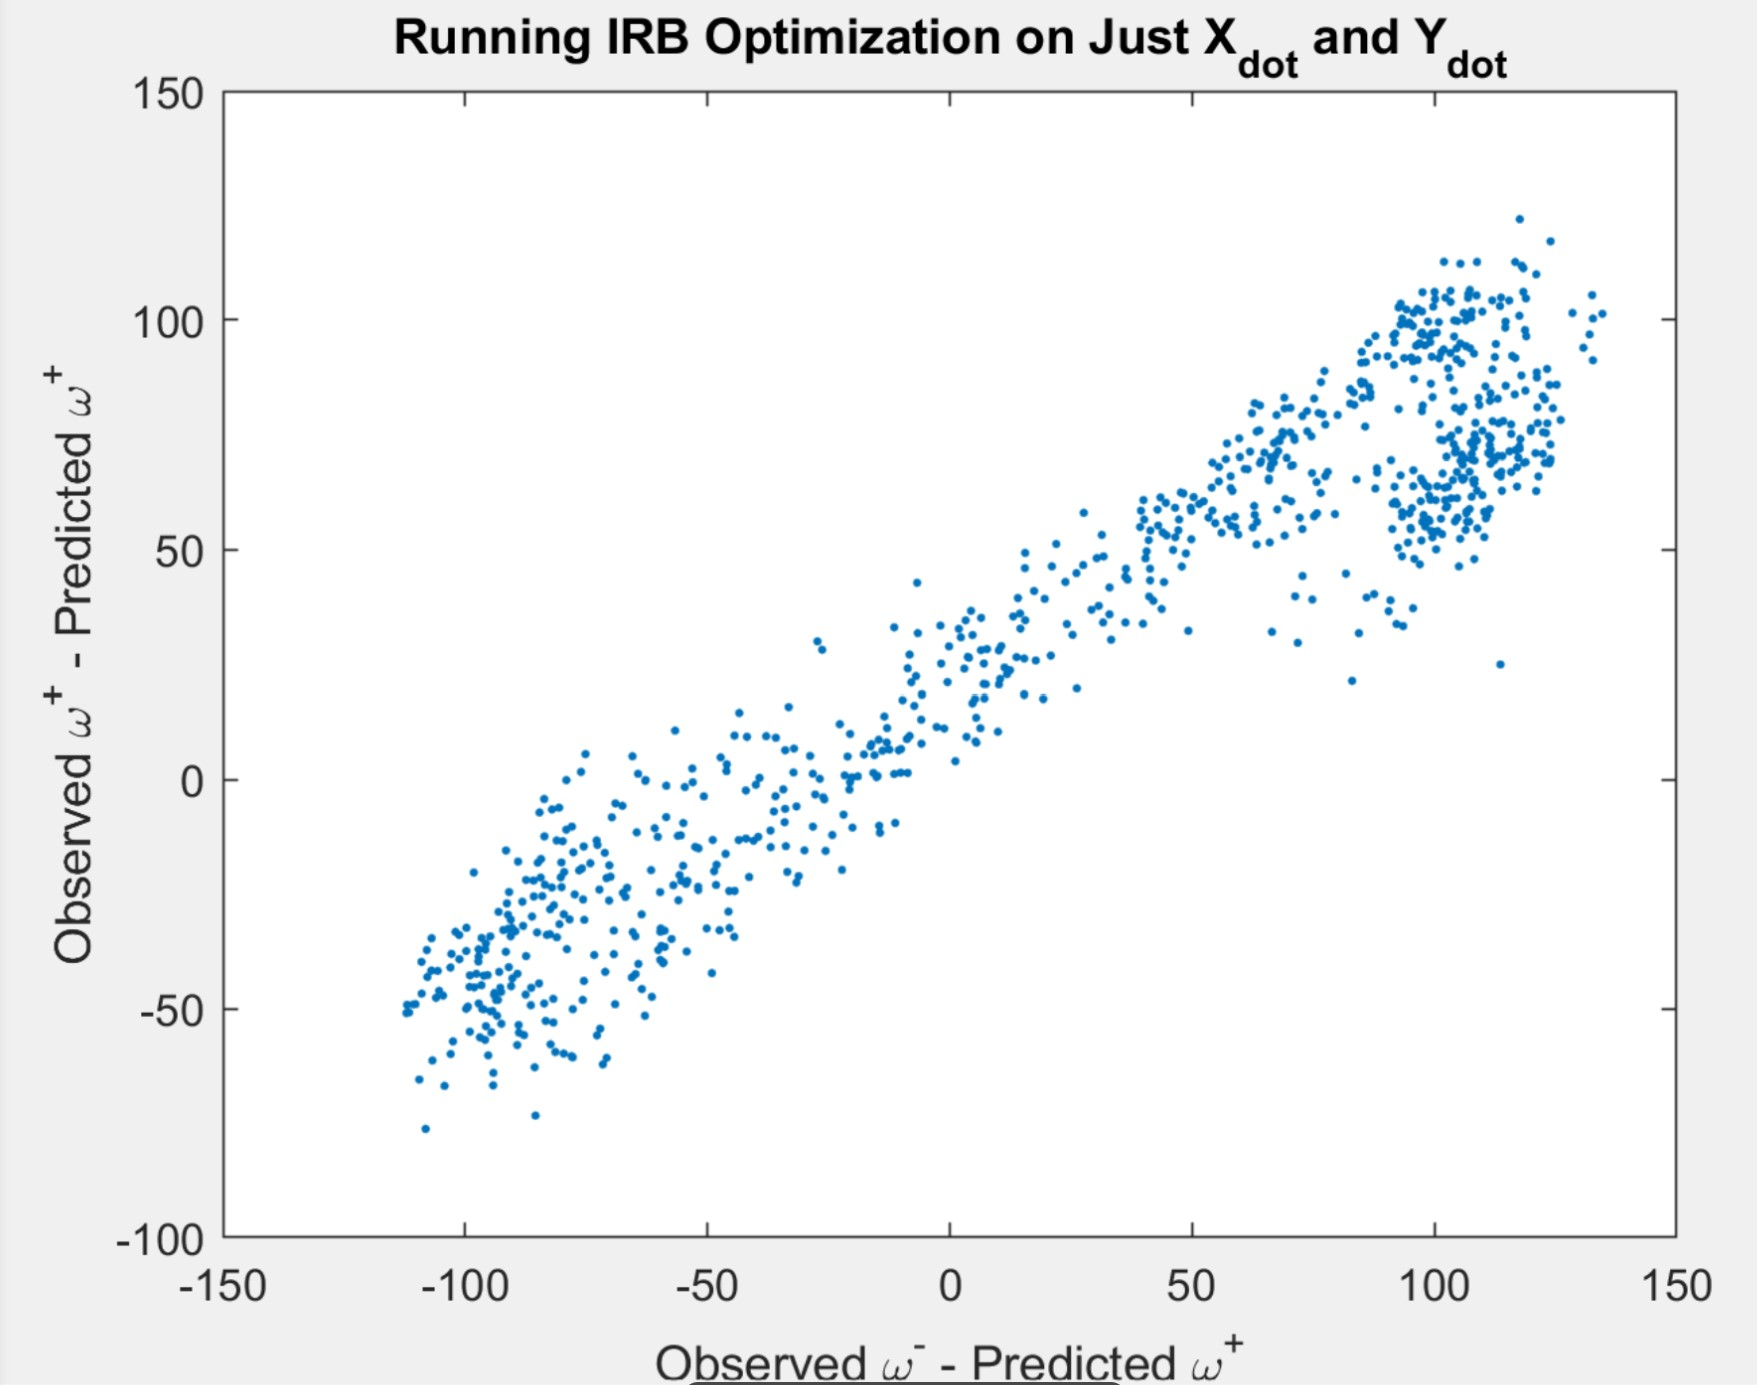
\includegraphics[scale=0.4]{redErr.jpg}
\label{fig:redErr}
\end{figure}


\section{Moment of Inertia}
One idea that Dr. Posa brought up last meeting was that perhaps, the benefit from adding a width element to the IRB model (less prediction error) could also simply be achieved by increasing the moment of Inertia. After some testing, any changes in the moment of inertia seemed to have super small effects on the error (Fig \ref{fig:incMOI}, Fig \ref{fig:decMOI}). This is something we still need to explore. 

\begin{figure}[ht]
    \caption{Varying Moment of Inertia}
    \centering
    \begin{subfigure}[b]{0.45\linewidth}
        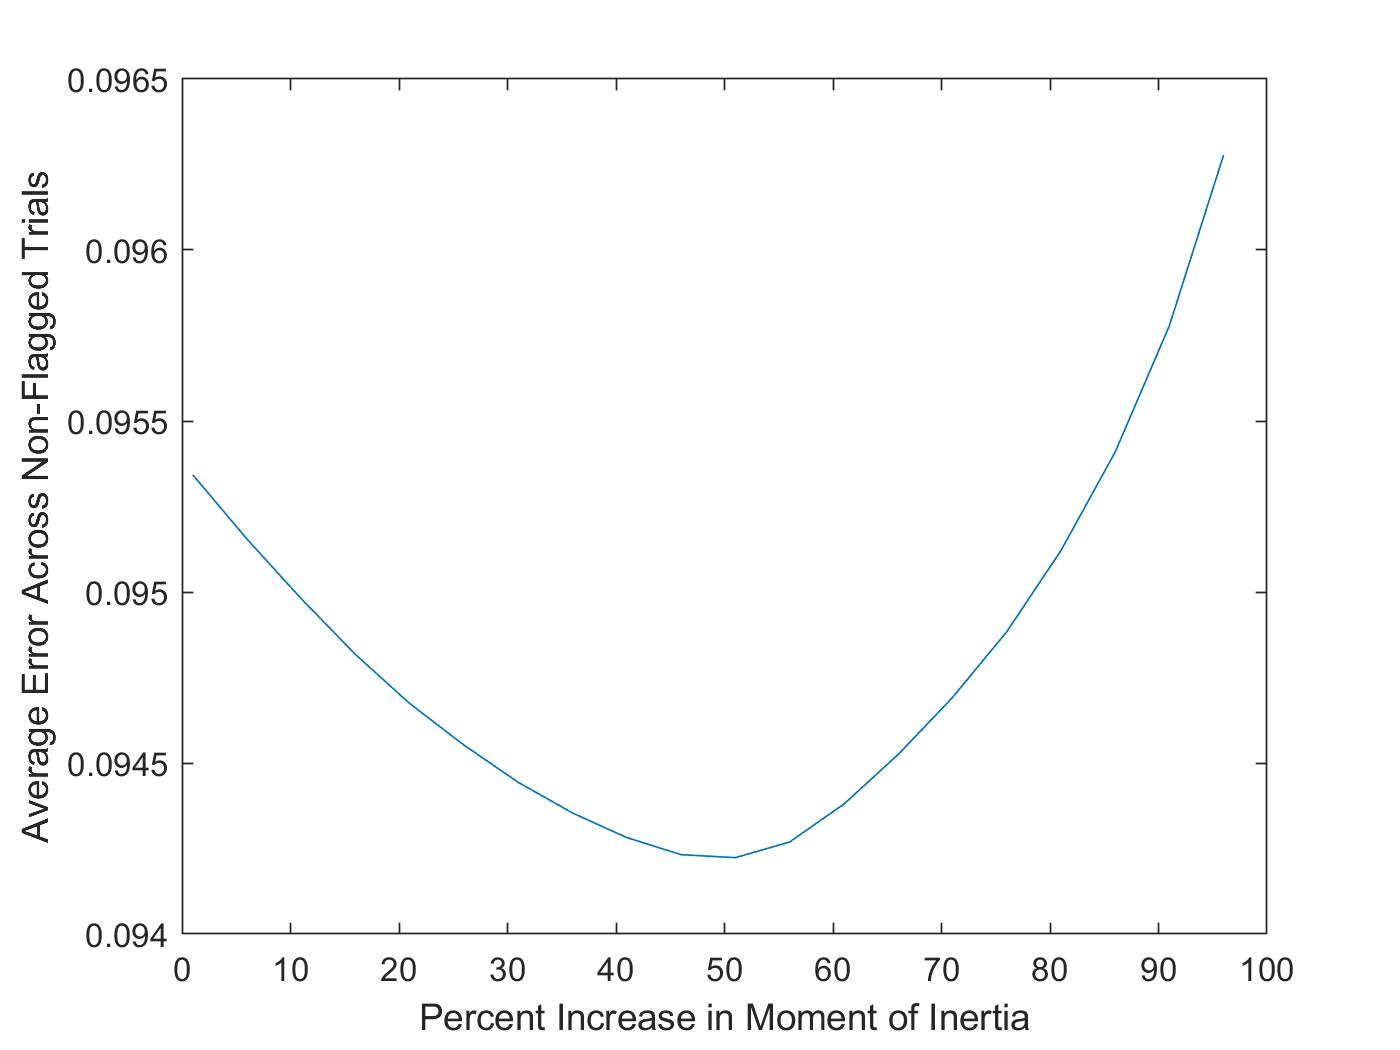
\includegraphics[scale=0.12]{incMOI.jpg}
        \caption{Increasing Moment of Inertia}
        \label{fig:incMOI}
    \end{subfigure}
    \quad
    \begin{subfigure}[b]{0.45\linewidth}
       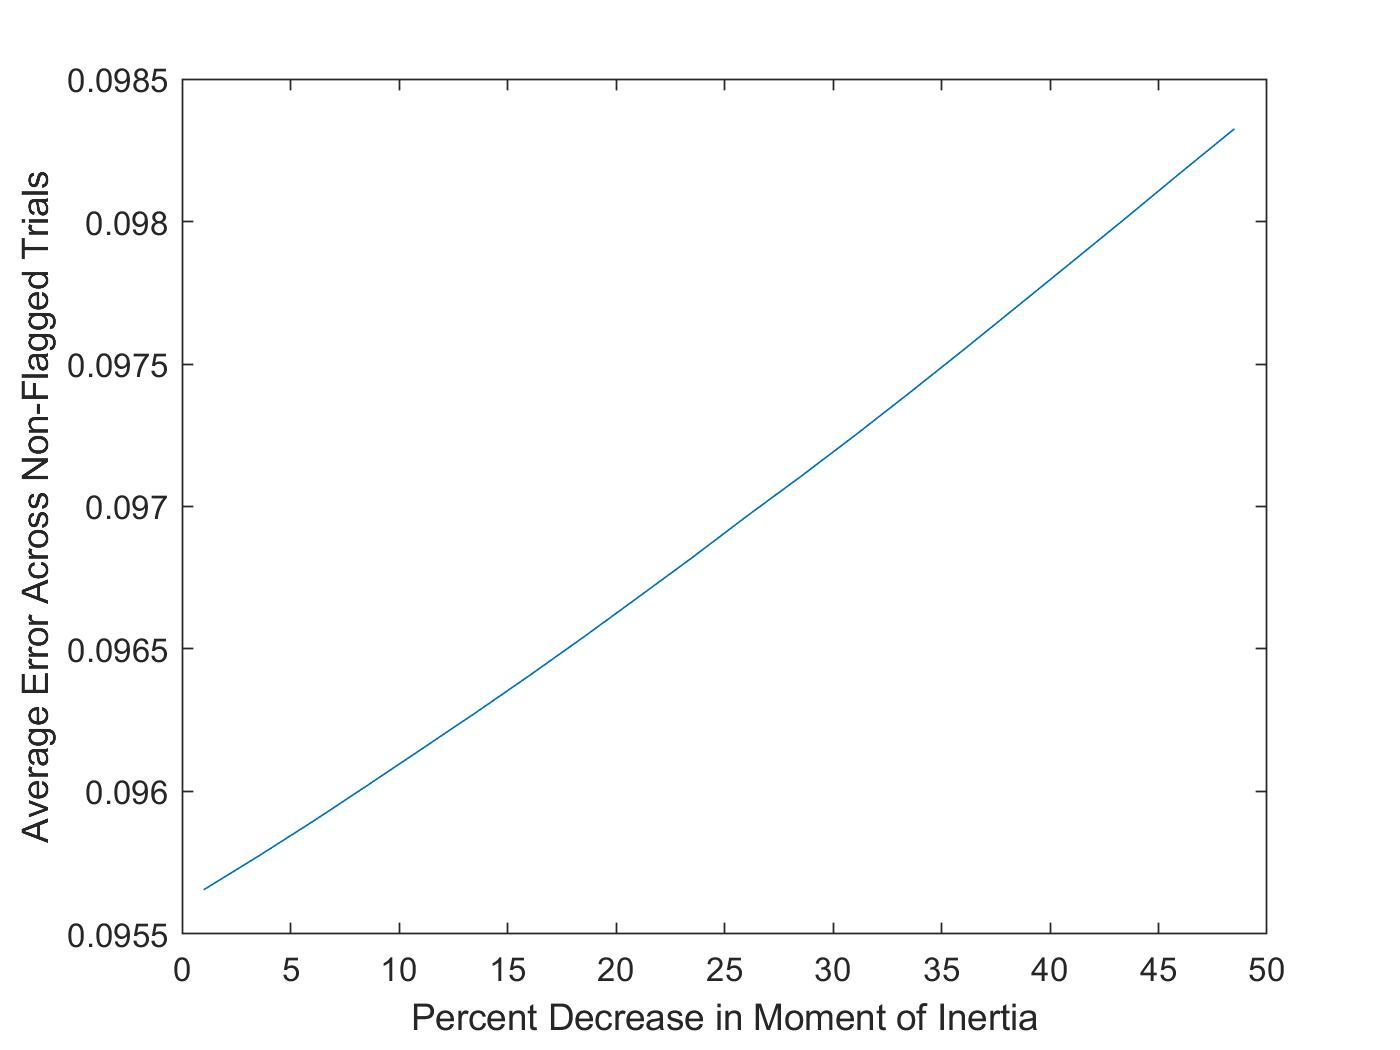
\includegraphics[scale=0.12]{decMOI.jpg}
        \caption{Decreasing Moment of Inertia}
        \label{fig:decMOI}
    \end{subfigure}
\end{figure}

\section{Trends}
The moment exerted on the body in the IRB with patch width model can be thought of as being comprised of three pieces. 
\begin{align}
    m_{net} = m_{tan} + m_{norm} + m_{width}
     \begin{cases}
       m_{tan} = P_t * y\\
       m_{norm} = P_n * x\\
       m_{width} = P_n * width\\
    \end{cases} 
\end{align}
 
 \noindent In the plot below (Fig \ref{fig:andy1}), we can see that a small $m_{net}$ has a larger expected error. The converse also stands, a larger $m_{net}$ corresponds to a smaller expected error. 
\begin{figure}[ht]
    \caption{Varying Moment of Inertia}
    \centering
    \begin{subfigure}[b]{0.45\linewidth}
        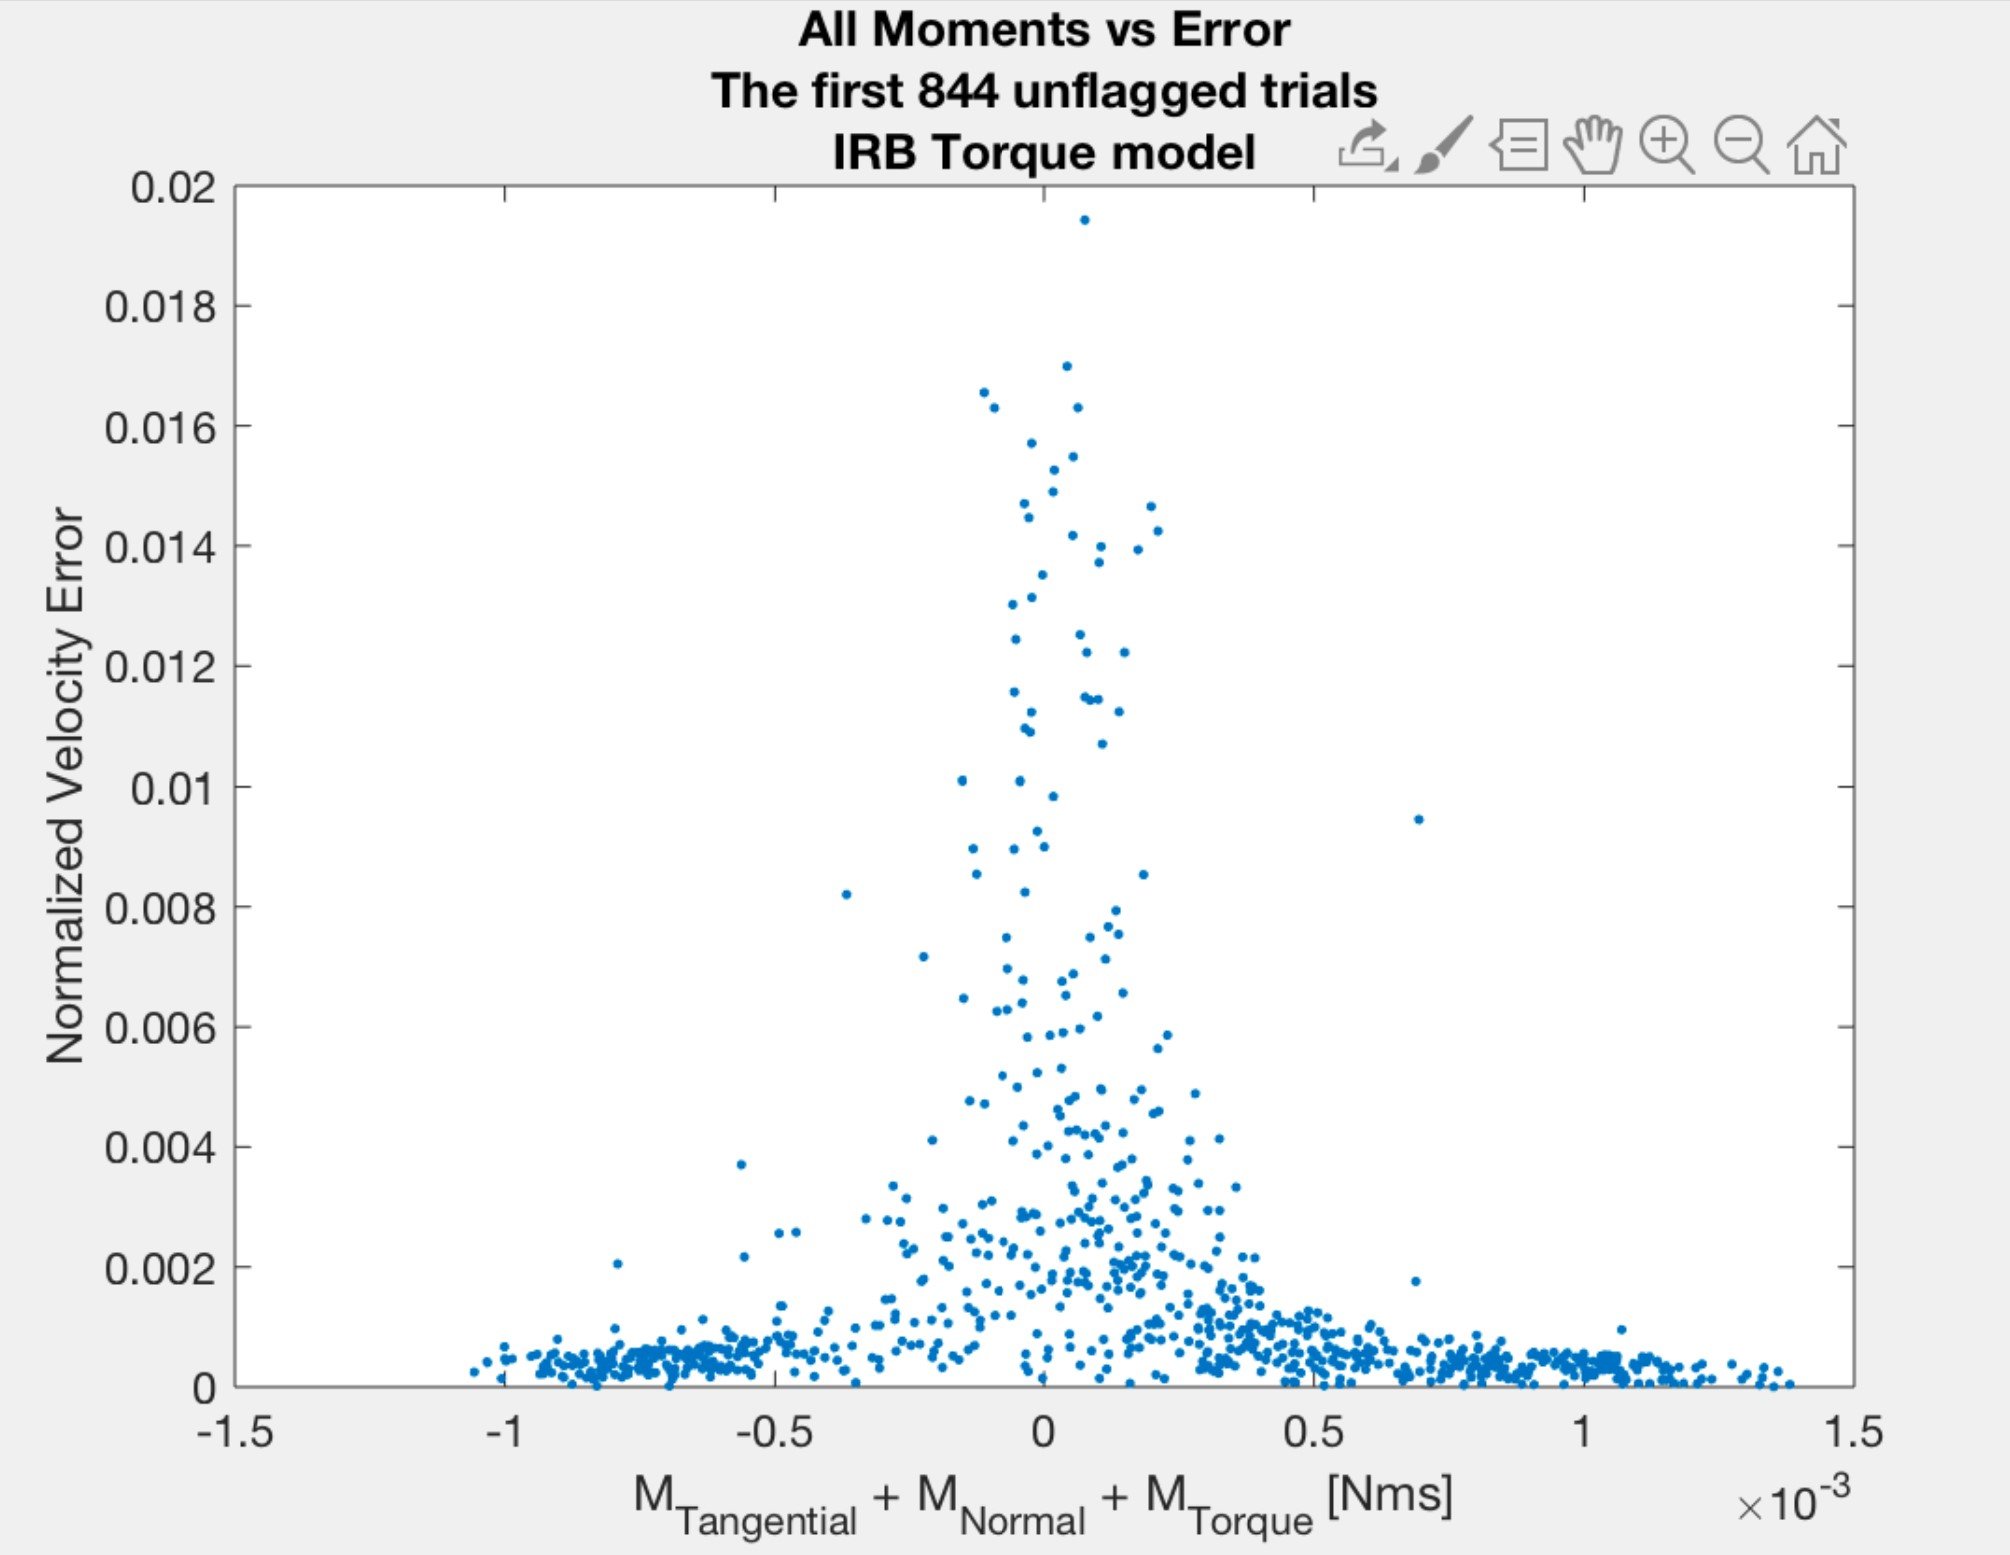
\includegraphics[scale=0.25]{andy1.jpg}
        \caption{Net Moments vs. Error}
        \label{fig:andy1}
    \end{subfigure}
    \quad
    \begin{subfigure}[b]{0.45\linewidth}
       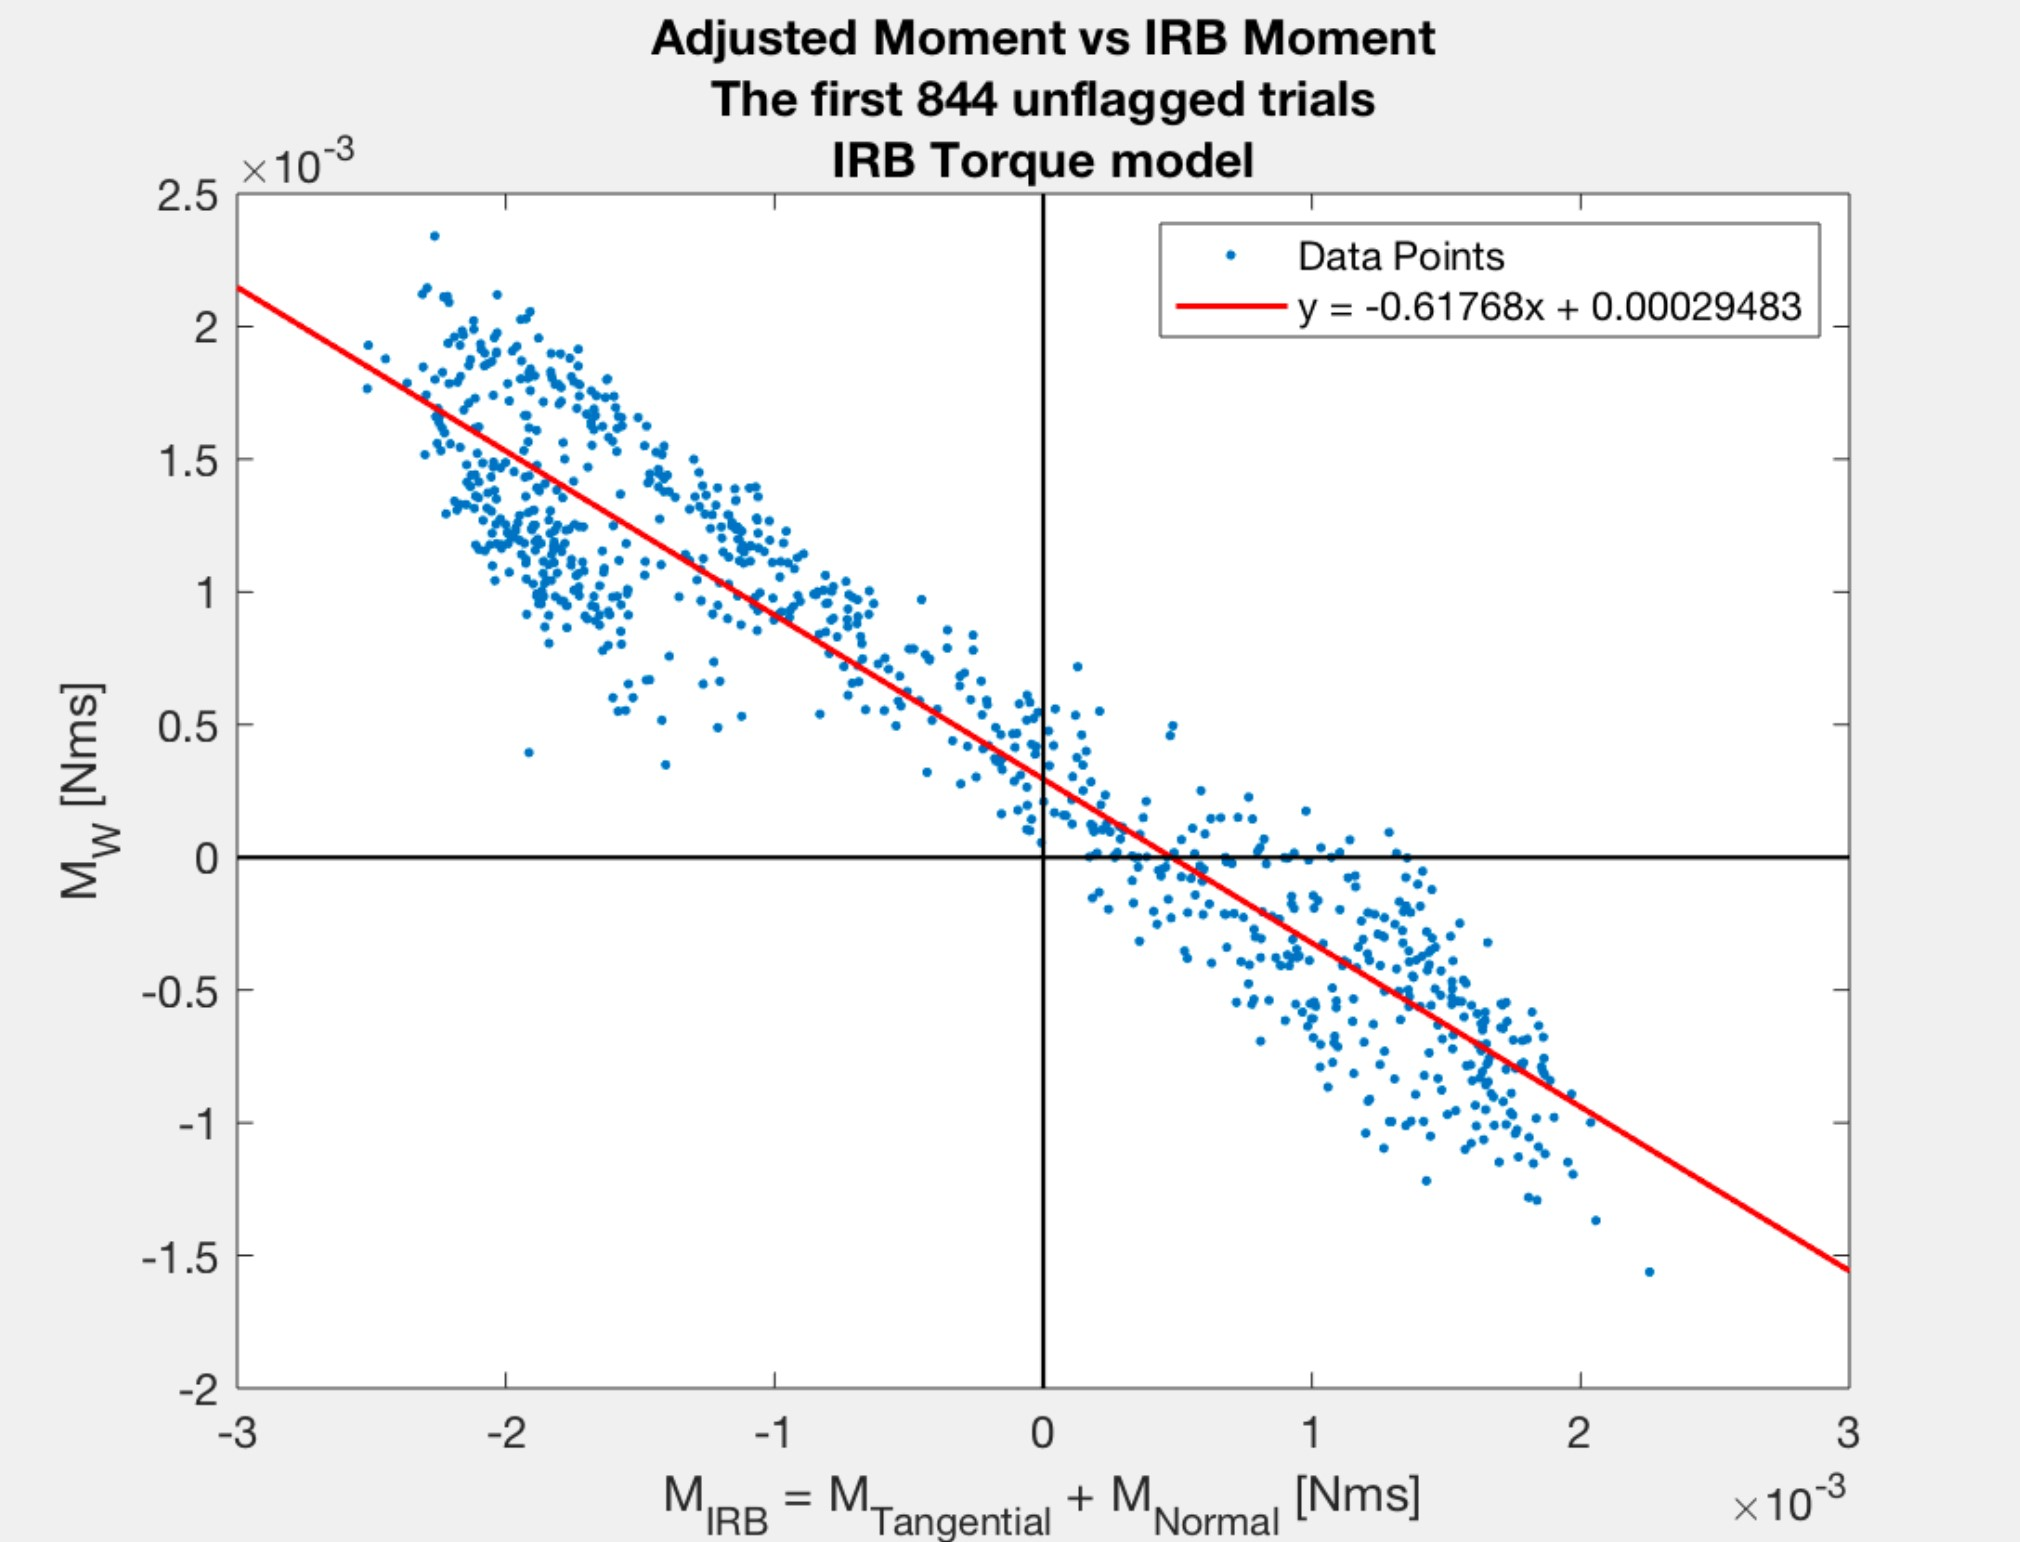
\includegraphics[scale=.25]{andy2.jpg}
        \caption{IRB Moment vs. Width Moment}
        \label{fig:andy2}
    \end{subfigure}
\end{figure}

\noindent The figure above (Fig. \ref{fig:andy2}) shows the relationship between the moment due to the base IRB model ($m_{IRB} = m_{tan} + m_{norm}$) and the moment due to the added patch size ($m_{width}$). The $m_{width}$ is in place to adjust for the error in the model. It turns out only when this torque is on average 60\% of the $m_{IRB}$ does it reduce the error of the model. This means that often the model tends to overestimate the torque from the width and thus overestimate the patch size.\\

\noindent The last relationship we examined was that between the net moment ($m_{net}$) and the moment due to the patch width ($m_{width}$). It seems to also follow a sinusoidal curve (Fig. \ref{fig:joah1}, below) and an early theory is that it has to do with how the moment is calculated from the Jacobian. 

\begin{figure}[t!]
\centering
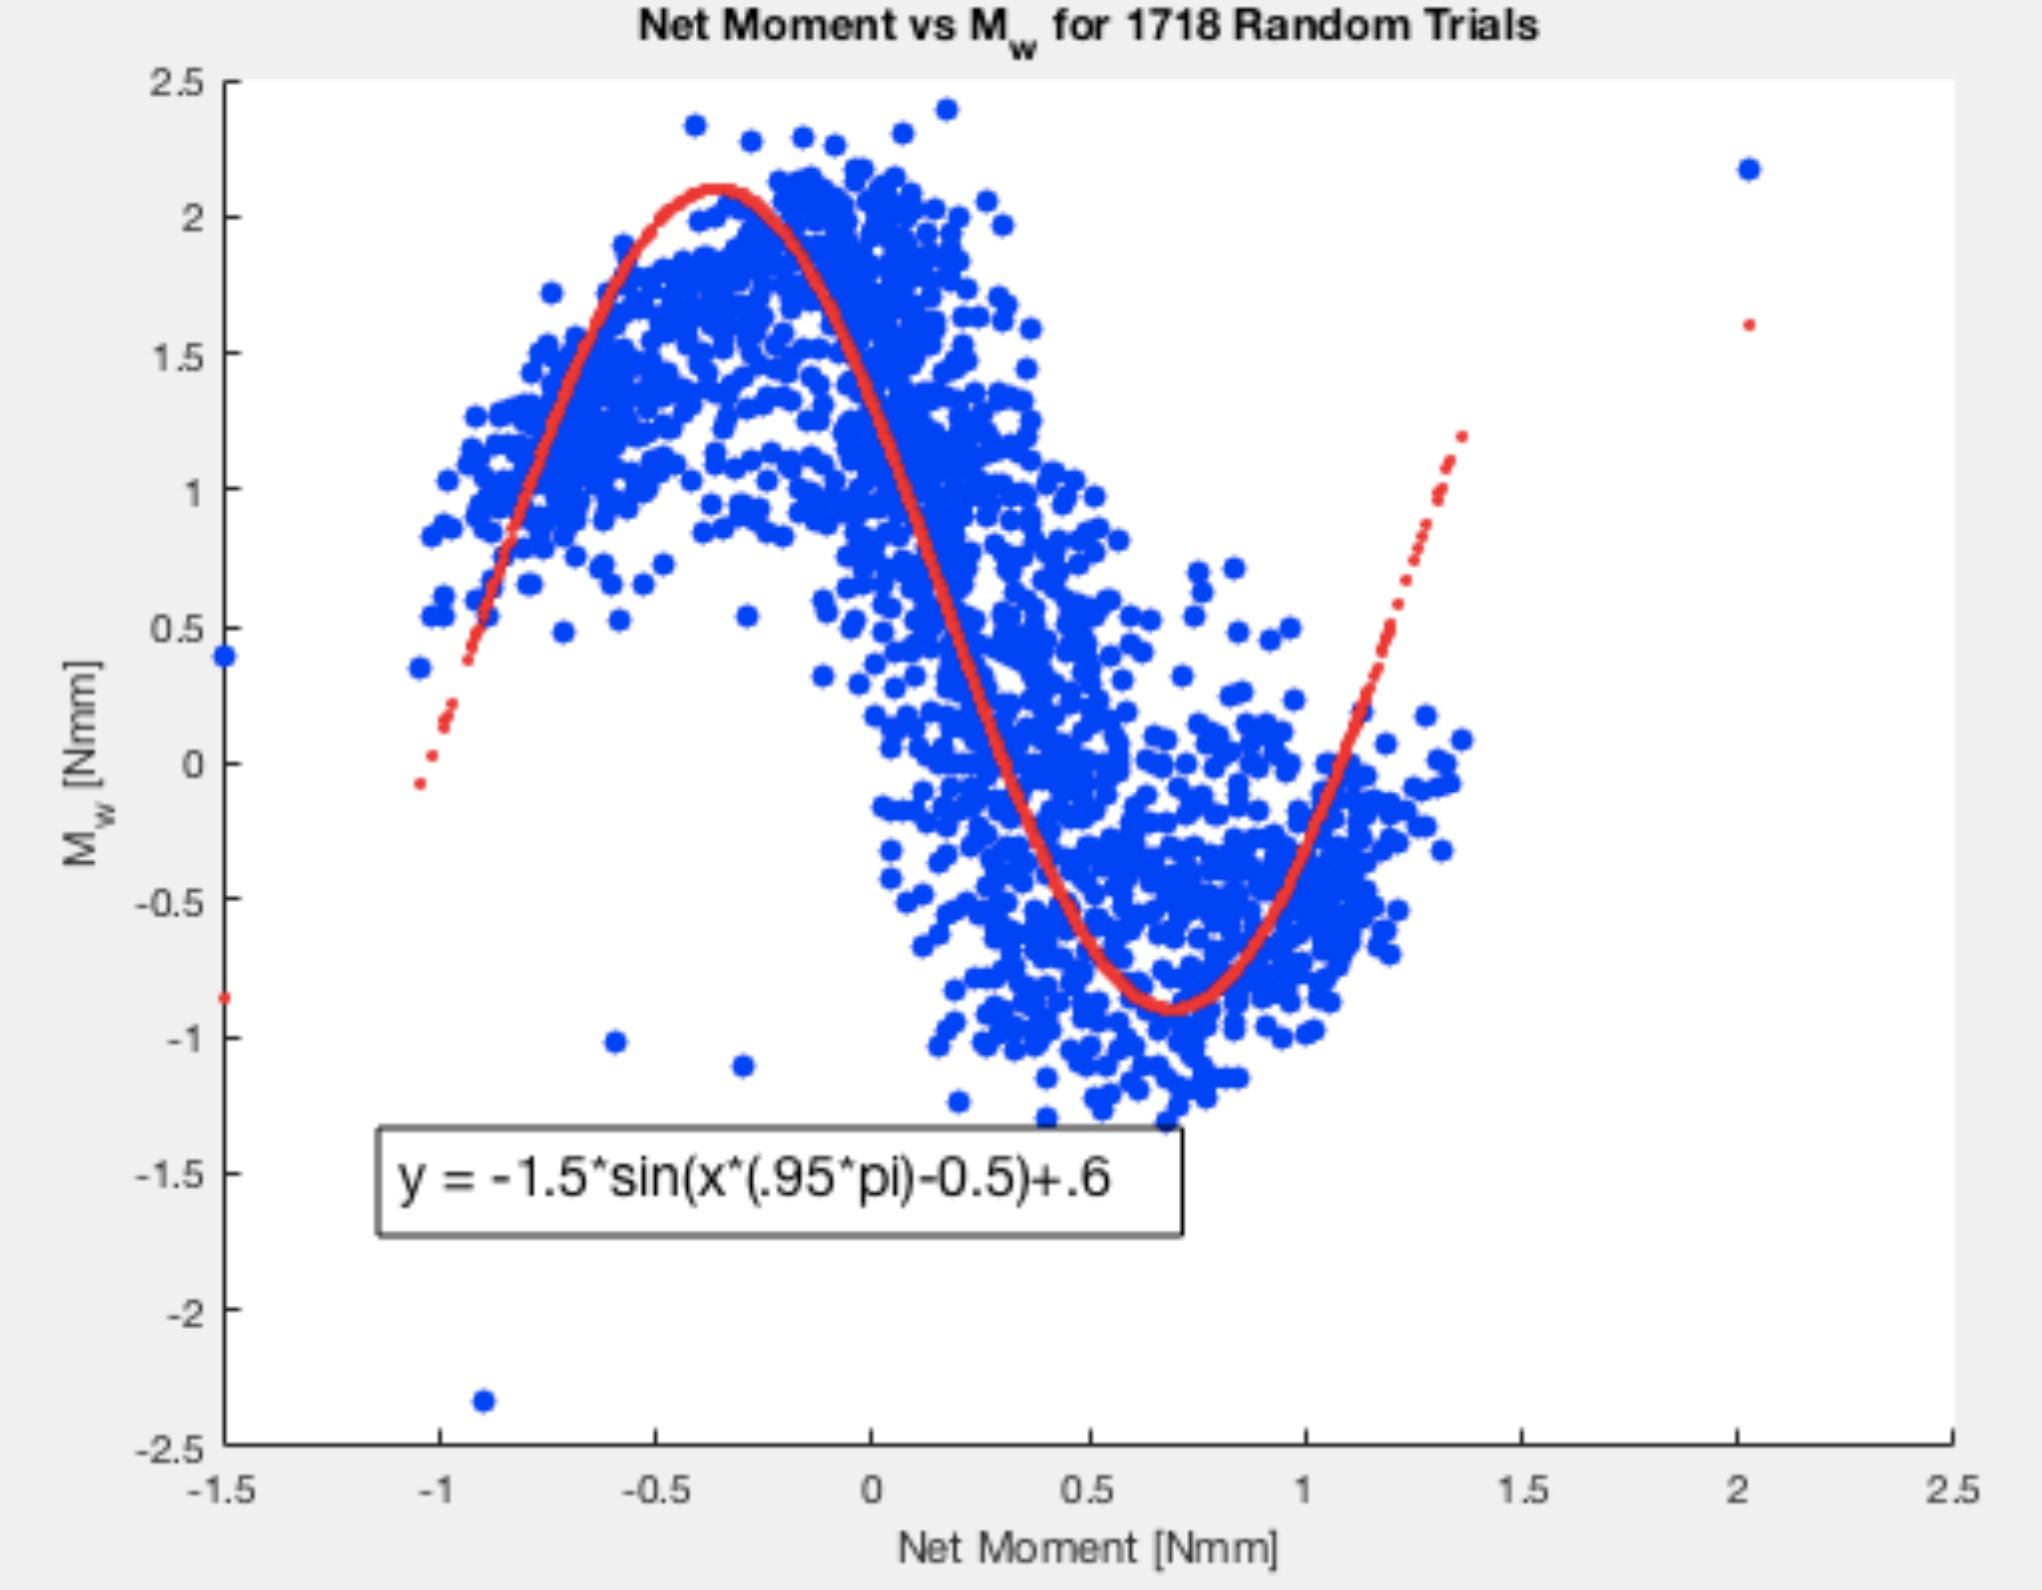
\includegraphics[scale=0.5]{Joah1.jpg}
\caption{Net Moment vs. Moment due to Width}
\label{fig:joah1}
\end{figure}

\end{document}
